% 第 8 章后半：PDF p.112--116（原书 p.104--108），前半见 ch08.tex
% ===== PDF p.112 (原书 p.104) =====
（接上页）因此，测地线全体相当于把 $T^{2}$ 考虑无限多个（对每个 $(a,b)\in\Z^{2}$ 各一个），即
\[ \bigoplus_{(a,b)\in\Z^{2}}H(T^{2}) . \]
（$T^{2}$ 的情形，所有测地线的长度都取局部极小，所以 Morse 指数是 0。）由此可知
\[ H(\Omega T^{2})\cong\bigoplus_{(a,b)\in\Z^{2}}H(T^{2}), \]
从而明白环路空间的同调与 Floer 同调不同。

\section{Floer 同调与变分问题}

要进一步弄清环路空间的同调与 Floer 同调不同的理由，必须更仔细地看看 $\mathfrak{H}$ 的变分问题。我们来研究泛函 (5)。为此，把 $\R^{2}$ 看作 $\C$，把 $p(t)+\sqrt{-1}q(t)$ 作 Fourier 展开。也就是说，设
\[ p(t)+\sqrt{-1}q(t)=\sum_{i=-\infty}^{\infty}a_it^{i} \tag{7} \]
（其中 $t$ 取遍单位圆，即 $t\in\{t\in\C\mid |t|=1\}$），这时
\[ \mathfrak{H}(p,q)=\sum_{i=-\infty}^{\infty}i\cdot a_i^{2} \tag{8} \]
可以通过计算确认。

打量式 (8)，就能看出泛函 $\mathfrak{H}$ 的样子。也就是说，$\mathfrak{H}$ 是 $q$ 的二次函数，特征值为正的方向有无限多个（对应 $i>0$），特征值为负的方向有无限多个（对应 $i<0$），此外特征值为 0 的方向有 2 个（对应 $i=0$）。也就是说，使泛函减少的方向有无限多个，因此 Morse 指数是无穷大。进一步说，全体之中只有一半是负特征值，所以应当说它是“二分之一的无穷大”吧。

如第 5 节所述，要求同调，只需按 Morse 指数把次数错开。即
\[ HF_d(T^{2})=H_{d+\frac{\infty}{2}}(\Omega T^{2}), \]

% ===== PDF p.113 (原书 p.105) =====
可以写成这样。（当然，这个式子并不具有严格数学的意义。）

在回到镜像对称的话题之前，先谈一谈 Floer 同调在辛几何中的应用。把 (4) 的泛函加入 Hamilton 函数 $H(t;q,p)$ 稍作变形，考虑泛函
% [Tutor Note: 原书此处引作（4），按上下文应为式（5）（p.103 中 $\mathfrak{H}$ 的定义式）；式（4）是 $\bigoplus_{k}H_{d-k}(\operatorname{Crit}_k(\mathfrak{L}))$。疑原书式号误，照原文录。]
\[ \mathfrak{H}_H(q,p)=\int_{t=0}^{t=1}\left(p(t)\frac{q(t)}{dt}+H(t;q(t),p(t))\right)dt \tag{9} \]
% [Tutor Note: 原书（9）的被积式同样印作 $\frac{q(t)}{dt}$；按通行记号应作 $\frac{dq(t)}{dt}$，与第 4 节 $\mathfrak{L}$ 的写法同此，照原文录。]
（$H$ 是 $S^{1}\times T^{2}$ 上的函数，也就是说，对 $t$ 也是周期的函数。）于是可知，$\mathfrak{H}_H$ 的临界点 $(q,p)$ 是 Hamilton 正则方程
\[ \frac{dq}{dt}=\frac{\partial H}{\partial p},\qquad \frac{dp}{dt}=-\frac{\partial H}{\partial q} \tag{10} \]
的周期解。由 (10) 的周期解的空间，同样可以定出 Floer 同调 $HF(T^{2})$；实际上可以知道，它与把 $H$ 取成 0 的情形是同一个同调群。

以上的考察对任何紧辛流形都成立；利用它，例如可以得到下面这样的定理。

\par\medskip\noindent\textbf{对任意紧相空间上周期的 Hamilton 函数 $H$，正则方程 (10) 都有周期解。}\par\medskip

这样的应用，正是 Floer 考虑 Floer 同调的动机。

再提一下与第 2 节的关系。$S^{1}$ 上的 Dirac 算子（这样说有点夸张）是 $\sqrt{-1}\,d/ds$（$t=s^{2\pi\sqrt{-1}s}$）。这时，特征函数分解就是 (7) 的 Fourier 级数，$i$ 是特征函数 $t^{i}$ 的特征值。也就是说，写成 (8) 那样时，二次形式的特征值就是 Dirac 算子的特征值。构成第 2 节“电子之海”的无限多个负能量所对应的自由度，对应于 Morse 指数，而它是二分之一的无穷大。
% [Tutor Note: 原书此处印作 $t=s^{2\pi\sqrt{-1}s}$，原书如此；按上下文（$t\in S^{1}$ 的参数化）疑为 $t=e^{2\pi\sqrt{-1}s}$ 之误，正文照录。]

与第 3 节佐藤 Grassmann 流形的关系，出现在 Floer 同调以及镜像对称与可积系统、D-模的关系之中。这一点本章无法涉及。

% ===== PDF p.114 (原书 p.106) =====
\section{Floer 同调与 Gromov--Witten 不变量}

Floer 同调与 Gromov--Witten 不变量之间有密切的关系。要说明这一点，必须就第 5 节提到的抵消再稍作补充。请看下面的图 2。

图 2 是把球面稍稍扭曲、使其有两个隆起，再把它放在 3 维空间中的图。设 $M$ 为图 2 的曲面，$f$ 为 $M$ 上的函数：对每个点，取该点的高度为函数值。于是 $f$ 有 4 个临界点 $p_1,p_2,q,r$。$p_1,p_2$ 的 Morse 指数是 2，$q$ 的 Morse 指数是 1，$r$ 的 Morse 指数是 0。由此，把相当于 (3) 的东西（用 $f$ 代替 $\mathfrak{L}$，用 $M$ 代替 $\Omega(S^{2})$）作出来，所得的是

\[
  C_i=\begin{cases}
    \Z & i=0,1,\\
    \Z\oplus\Z & i=2,\\
    0 & \text{其他}.
  \end{cases}
\]

$C_i$ 比 $M$ 的 $i$ 次同调（也就是球面的 $i$ 次同调）$H_i(M)$ 大，而 $H_i(M)$ 是

\[
  H_i(M)=\begin{cases}
    \Z & i=2,\\
    0 & \text{其他}.
  \end{cases}
\]

\begin{figure}[htbp]
  \centering
  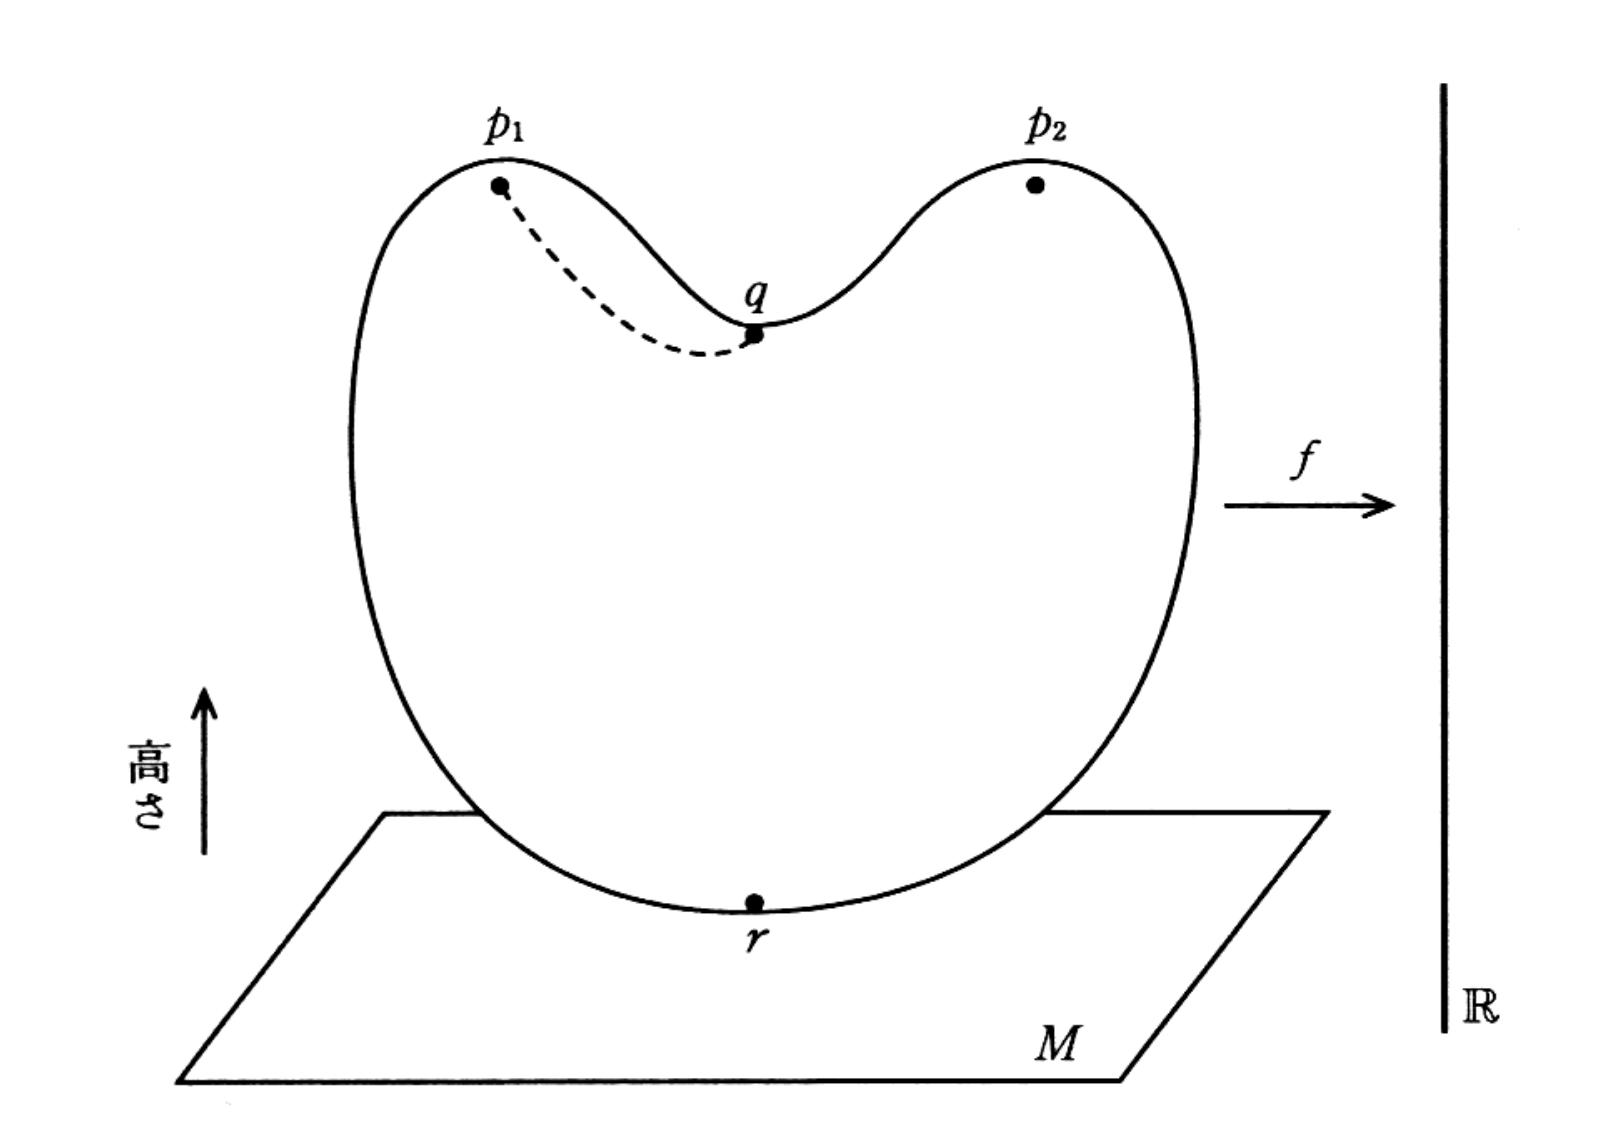
\includegraphics[width=0.62\linewidth]{figures/ch08-fig2.png}
  \figtitle{2}{把球面稍稍扭曲、使其有两个隆起的曲面 $M$，以及表示高度的函数 $f$；$p_1,p_2$ 的 Morse 指数为 2，$q$ 为 1，$r$ 为 0（原书 p.106）}
\end{figure}

下面说明由 $C_i$ 通过抵消得到 $H_i(M)$ 的机制。

% ===== PDF p.115 (原书 p.107) =====
考虑 $f$ 的梯度向量场 $\operatorname{grad} f$。（$\operatorname{grad}_p f$ 是在 $p$ 处指向 $f$ 增加最快的方向的向量。）从 $p_1$ 出发，沿 $-\operatorname{grad} f$ 的方向移动点。于是，如图 2 的虚线所示，恰好有一条从 $p_1$ 出发、在 $q$ 结束的曲线。这条曲线称为 $-\operatorname{grad} f$ 的积分曲线。当从 $p_1$ 出发、在 $q$ 结束的 $-\operatorname{grad} f$ 的积分曲线的条数为 1 时，定义

\[
  \langle \partial[p_1],[q]\rangle = 1 .
\]

这个 $\partial$ 称为边界算子。边界算子满足 $\partial\circ\partial=0$，在 $\bigoplus_i C_i$ 上定出链复形的结构，其同调群就是 $H(M)$。

也就是说，梯度向量场的积分曲线的条数，决定了临界点如何相互抵消而给出同调群。

从有限维的情形，转到第 6 节、第 7 节所述 Floer 同调的情形。下面的事实 (*) 是 Floer 发现 Floer 同调的关键。

\par\medskip\noindent\textbf{(*) 泛函 $\mathfrak{L}$ 的梯度向量场的积分曲线，就是全纯映射 $S^{1}\times\R\to M$。}\par\medskip

下面说明 (*)。$\mathfrak{L}$ 是第 4 节 (5) 那样的泛函。它的积分曲线是映射 $\R\to\Omega M$，但可以看作映射 $\R\times S^{1}\to M$。$\R\times S^{1}$ 与复平面去掉原点后的集合可以等同，因此可以定义“映射 $\R\times S^{1}\to M$ 是全纯映射（也就是复解析的）”。(*) 说的是：$\R\times S^{1}\to M$ 是 $\mathfrak{L}$ 的积分曲线，与对应的 $\R\times S^{1}\to M$ 是全纯映射，这两件事等价。\footnote{把环路空间的点看作弦，则弦的时间演化即环路空间上的道路可以看作从曲面出发的映射——这是弦理论的基本想法。另外，“从曲面出发的映射是全纯映射”这一方程（即 Cauchy--Riemann 方程）可以看作弦理论的运动方程。}
% [Tutor Note: 原书此处印作「4 節の(5)」；式（5）在第 6 节且为 $\mathfrak{H}$，而 $\mathfrak{L}$ 在第 4、5 节中没有编号式。疑原书节号与式号均有误，照原文录。]

那么，来回忆本节前半所述的内容。那里说的是：要从“临界点”导出“同调”，必须考虑“临界点的抵消”。抵消的情形，由泛函的梯度向量场的积分曲线的条数决定。
% ===== PDF p.116 (原书 p.108) =====
而且，由 (*) 可知，在 $\mathfrak{L}$ 的情形，梯度向量场的积分曲线正是全纯映射 $\R\times S^{1}\to M$。

至此，Floer 同调与 Gromov--Witten 不变量之间就联系起来了。也就是说，要从“Hamilton 力学系的周期点”导出“Floer 同调”，必须考虑用“全纯映射的条数”来做的抵消——就是这个意思。而所谓全纯映射的条数，正是 Gromov--Witten 不变量。

上面的说明有一处含糊：其实，只要把 Floer 同调作为群（或者向量空间）来考虑，“抵消”就不会发生。\footnote{环路空间，也就是闭弦（closed string）的情形。开弦（open string）时会发生。}也就是说，

\[ HF(M)=H(M) \tag{11} \]

全纯映射的效果，一旦考虑积就会显现出来。例如，量子上同调定出 $H(M)$ 上的积结构，\footnote{把通常上同调的杯积作“量子形变”所得的东西。}但与其那样理解，不如认为它是通过 (11) 得到的 $HF(M)$ 上的上同调，这样反而更自然。

% [Tutor Note: 原书此句作「$HF(M)$ 上のコホモロジー」，字面照录；$HF(M)$ 本身是 Floer 同调群，作者此说或指通过 (11) 在其上读出的量子上同调结构。]

% [Tutor Note: 原书章末附有作者姓名的假名读音标记；译文按全书体例省略，作者名已在章首署名中给出。]

\begin{reflist}
  \item[{[1]}] 深谷賢治，『解析力学と微分形式』，岩波書店，2004 年。
  \item[{[2]}] http://www.math.kyoto-u.ac.jp/\~{}fukaya/ 上载有 1997 年静冈大学的讲义录（由横山美佐子记录）。
  \item[{[3]}] 深谷賢治，『シンプレクティック幾何学』（岩波講座·現代数学の展開），岩波書店，1999 年。
  \item[{[4]}] 佐藤幹夫（著），野海正俊（記），『ソリトン方程式とグラスマン多様体』，上智大学数学講究録 18，1984 年。
\end{reflist}

% 章末恢复全书默认的罗马数字节号（本章开头曾按原书改为阿拉伯数字）
\renewcommand{\thesection}{\Roman{section}}

